%  FICHIER  :   template_fira_two_cols.tex
%  A copier à côté des autres .tex et à déclarer dans config.json
% ------------------------------------------------------------------
\documentclass[11pt,a4paper]{article}

% ─── pack de base ─────────────────────────────────────────────────
\usepackage[T1]{fontenc}
\usepackage[utf8]{inputenc}
\usepackage{textcomp}
\usepackage{newtxtext}
\usepackage[british]{babel}
\usepackage[left=0mm,right=0mm,top=0mm,bottom=0mm]{geometry}
\usepackage[stretch=25,shrink=25,tracking=true,letterspace=30]{microtype}
\usepackage{graphicx,xcolor,marvosym,enumitem,paracol,hyperref}
\usepackage{FiraSans}
\renewcommand{\familydefault}{\sfdefault}
\usepackage{array} 
\usepackage{tabularx}
\usepackage{ragged2e}
 \usepackage{fontawesome}
% ─── couleurs & listes ────────────────────────────────────────────
\definecolor{cvblue}{HTML}{304263}
\setlist{parsep=0pt,topsep=0pt,partopsep=1pt,itemsep=1pt,leftmargin=6mm}
\hypersetup{colorlinks=true,urlcolor=white,linkcolor=white}

% ─── macros maison (identiques au modèle original) ────────────────
\newcommand{\dates}[1]{\hfill\textbf{#1}}
\newcommand{\is}{\par\vskip.5ex plus .4ex}
\newcommand{\smaller}[1]{{\small$\diamond$\ #1}}
\newcommand{\headleft}[1]{\vspace*{3ex}\textsc{\textbf{#1}}\par%
  \vspace*{-1.5ex}\hrulefill\par\vspace*{0.7ex}}
\newcommand{\headright}[1]{\vspace*{2.5ex}\textsc{\Large\color{cvblue}#1}\par%
  \vspace*{-2ex}{\color{cvblue}\hrulefill}\par}

% ─── défaut de secours si sidetext absent dans d’autres modèles ───
\providecolor{sidetext}{rgb}{0,0,0}
\definecolor{maincolor}{HTML}{ffffff}
% ─────────────────────────── DOCUMENT ─────────────────────────────
\begin{document}
\thispagestyle{empty}
\setlength{\topskip}{0pt}\setlength{\parindent}{0pt}\setlength{\parskip}{0pt}
\raggedbottom

\begin{minipage}[t]{0.33\textwidth}
  % Bande bleue d’en-tête
  \colorbox{cvblue}{\begin{minipage}[t][5mm][t]{\textwidth}\null\end{minipage}}
  \vspace{-.2ex}
  \colorbox{cvblue!90}{%
    \color{white}\kern0.09\textwidth
    \begin{minipage}[t][293mm][t]{0.82\textwidth}\raggedright
      \vspace*{2.5ex}
      % -------- Identité ------------------------------------------
      \Large MOUROUVIN Judikael\normalsize

      % Photo (s’affiche seulement si f223cf49699244c9a04d41d6a96ceaa3.png ≠ vide)
      \ifx\relaxf223cf49699244c9a04d41d6a96ceaa3.png\relax\else
        \vspace{2ex}\null\hfill
        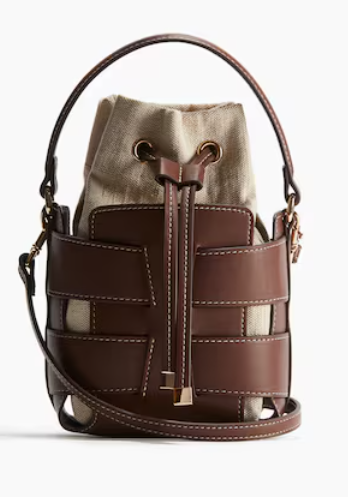
\includegraphics[width=0.4\textwidth]{f223cf49699244c9a04d41d6a96ceaa3.png}
        \hfill\null
      \fi

      % -------- Profil -------------------------------------------
      \headleft{Profil}
      \begingroup           % ouvre un groupe local
         % rétablit la justification pleine
        Passionné par l’informatique et le marketing digital, je possède une expérience solide en support technique, maintenance et gestion de projets numériques. Mon alternance à la DSI de la Mairie du Gosier a renforcé mon sens du service utilisateur et de l’exigence de résultat. Rigoureux et réactif, j’identifie rapidement les incidents et propose des solutions adaptées. Je souhaite désormais mettre ces compétences au service de nouveaux projets à temps plein.
      \endgroup             % referme : on revient à \raggedright

      % -------- Contact ------------------------------------------
      \headleft{Contact}\small
      \MVAt\  \texttt{jkmou971@gmail.com}\par
      \Mobilefone\ +590 0690 91 14 48\par
      \Letter\ Route de Cocoyer\par
      97190 Gosier\par
      \faLinkedin\  \href{}{}
      \normalsize

      % -------- Langues (si dispo) -------------------------------
      \ifx\relax\begin{itemize}[leftmargin=*]
\item English - \textcolor{gray}{}
\item Espagnol - \textcolor{gray}{}\end{itemize}\relax\else
        \headleft{Langues}
        \begin{itemize}[leftmargin=*]
\item English - \textcolor{gray}{}
\item Espagnol - \textcolor{gray}{}\end{itemize}
      \fi

      % -------- Compétences --------------------------------------
      \headleft{Compétences}
      \begin{itemize}[leftmargin=*]
\item Administration
\item Réseaux
\item Support
\item Maintenance
\item Configuration
\item Marketing
\item Digital\end{itemize}

      % -------- Centres d’intérêt --------------------------------
      \headleft{Intérêts}
      \begin{itemize}[leftmargin=*]
\item Lecture
\item Sport
\item Musique
\item Voyage
\end{itemize}

    \end{minipage}\kern0.09\textwidth
  }
\end{minipage}
% ================================================================
\hskip2.5em
% ======================= COLONNE DROITE =========================
\begin{minipage}[t]{0.56\textwidth}
  \setlength{\parskip}{0.8ex}
  \vspace{2ex}

  % ---------- EXPERIENCE ----------------------------------------
  \headright{Expérience}
  \colorbox{maincolor}{%
  \begin{minipage}{\linewidth}
    \noindent
    \textbf{Alternant en marketing digital}\hfill 09/2023 - 08/2024\\
    Mairie du Gosier, DSI\\[-0.3em]
    \begin{itemize}[leftmargin=*]
      \item Pilotage et déploiement de projets numériques pour les services municipaux. \item Analyse des besoins utilisateurs et mise en œuvre de solutions améliorant la productivité. \item Support technique, formation des agents et contribution à la stratégie digitale.
    \end{itemize}
  \end{minipage}}

\vspace{3mm}

\colorbox{maincolor}{%
  \begin{minipage}{\linewidth}
    \noindent
    \textbf{Animateur de la zone informatique}\hfill 10/2022 - 07/2023\\
    Pôle emploi, Gosier\\[-0.3em]
    \begin{itemize}[leftmargin=*]
      \item Assistance utilisateurs et résolution d’incidents postes de travail, réduisant les interruptions. \item Configuration et maintenance du parc informatique pour garantir la disponibilité. \item Diagnostic et réparation des pannes matérielles, accélérant la remise en service.
    \end{itemize}
  \end{minipage}}

\vspace{3mm}

\colorbox{maincolor}{%
  \begin{minipage}{\linewidth}
    \noindent
    \textbf{Stagiaire informaticien}\hfill 05/2020 - 08/2021\\
    Numerika, Baie-Mahault\\[-0.3em]
    \begin{itemize}[leftmargin=*]
      \item Configuration et maintenance de postes et périphériques, améliorant la stabilité. \item Support de proximité aux utilisateurs, accélérant la résolution quotidienne des incidents.
    \end{itemize}
  \end{minipage}}        % ← déjà formaté par build_placeholders()

  % ---------- EDUCATION -----------------------------------------
  \headright{Formation}
  \colorbox{maincolor}{%
  \begin{minipage}{\linewidth}
    \noindent
    \textbf{Bachelor Marketing Digital}\hfill 09/2023 - 08/2024\\
    CFA IUTS\\[-0.3em]
    \begin{itemize}[leftmargin=*]
      \item Fondamentaux du marketing en ligne et des réseaux sociaux. \item Gestion de projet digital et analyse de performance. \item Création de contenu et optimisation de la visibilité.
    \end{itemize}
  \end{minipage}}

\vspace{3mm}

\colorbox{maincolor}{%
  \begin{minipage}{\linewidth}
    \noindent
    \textbf{BTS Systèmes numériques option informatique et réseaux}\hfill 09/2019 - 06/2021\\
    Lycée Chevalier Saint-Georges, Abymes\\[-0.3em]
    \begin{itemize}[leftmargin=*]
      \item Architectures réseaux et systèmes d’exploitation. \item Maintenance et assistance technique. \item Initiation à la cybersécurité et au diagnostic matériel.
    \end{itemize}
  \end{minipage}}

\end{minipage}

\end{document}
